\documentclass[1p]{elsarticle_modified}
%\bibliographystyle{elsarticle-num}

%\usepackage[colorlinks]{hyperref}
%\usepackage{abbrmath_seonhwa} %\Abb, \Ascr, \Acal ,\Abf, \Afrak
\usepackage{amsfonts}
\usepackage{amssymb}
\usepackage{amsmath}
\usepackage{amsthm}
\usepackage{scalefnt}
\usepackage{amsbsy}
\usepackage{kotex}
\usepackage{caption}
\usepackage{subfig}
\usepackage{color}
\usepackage{graphicx}
\usepackage{xcolor} %% white, black, red, green, blue, cyan, magenta, yellow
\usepackage{float}
\usepackage{setspace}
\usepackage{hyperref}

\usepackage{tikz}
\usetikzlibrary{arrows}

\usepackage{multirow}
\usepackage{array} % fixed length table
\usepackage{hhline}

%%%%%%%%%%%%%%%%%%%%%
\makeatletter
\renewcommand*\env@matrix[1][\arraystretch]{%
	\edef\arraystretch{#1}%
	\hskip -\arraycolsep
	\let\@ifnextchar\new@ifnextchar
	\array{*\c@MaxMatrixCols c}}
\makeatother %https://tex.stackexchange.com/questions/14071/how-can-i-increase-the-line-spacing-in-a-matrix
%%%%%%%%%%%%%%%

\usepackage[normalem]{ulem}

\newcommand{\msout}[1]{\ifmmode\text{\sout{\ensuremath{#1}}}\else\sout{#1}\fi}
%SOURCE: \msout is \stkout macro in https://tex.stackexchange.com/questions/20609/strikeout-in-math-mode

\newcommand{\cancel}[1]{
	\ifmmode
	{\color{red}\msout{#1}}
	\else
	{\color{red}\sout{#1}}
	\fi
}

\newcommand{\add}[1]{
	{\color{blue}\uwave{#1}}
}

\newcommand{\replace}[2]{
	\ifmmode
	{\color{red}\msout{#1}}{\color{blue}\uwave{#2}}
	\else
	{\color{red}\sout{#1}}{\color{blue}\uwave{#2}}
	\fi
}

\newcommand{\Sol}{\mathcal{S}} %segment
\newcommand{\D}{D} %diagram
\newcommand{\A}{\mathcal{A}} %arc


%%%%%%%%%%%%%%%%%%%%%%%%%%%%%5 test

\def\sl{\operatorname{\textup{SL}}(2,\Cbb)}
\def\psl{\operatorname{\textup{PSL}}(2,\Cbb)}
\def\quan{\mkern 1mu \triangleright \mkern 1mu}

\theoremstyle{definition}
\newtheorem{thm}{Theorem}[section]
\newtheorem{prop}[thm]{Proposition}
\newtheorem{lem}[thm]{Lemma}
\newtheorem{ques}[thm]{Question}
\newtheorem{cor}[thm]{Corollary}
\newtheorem{defn}[thm]{Definition}
\newtheorem{exam}[thm]{Example}
\newtheorem{rmk}[thm]{Remark}
\newtheorem{alg}[thm]{Algorithm}

\newcommand{\I}{\sqrt{-1}}
\begin{document}

%\begin{frontmatter}
%
%\title{Boundary parabolic representations of knots up to 8 crossings}
%
%%% Group authors per affiliation:
%\author{Yunhi Cho} 
%\address{Department of Mathematics, University of Seoul, Seoul, Korea}
%\ead{yhcho@uos.ac.kr}
%
%
%\author{Seonhwa Kim} %\fnref{s_kim}}
%\address{Center for Geometry and Physics, Institute for Basic Science, Pohang, 37673, Korea}
%\ead{ryeona17@ibs.re.kr}
%
%\author{Hyuk Kim}
%\address{Department of Mathematical Sciences, Seoul National University, Seoul 08826, Korea}
%\ead{hyukkim@snu.ac.kr}
%
%\author{Seokbeom Yoon}
%\address{Department of Mathematical Sciences, Seoul National University, Seoul, 08826,  Korea}
%\ead{sbyoon15@snu.ac.kr}
%
%\begin{abstract}
%We find all boundary parabolic representation of knots up to 8 crossings.
%
%\end{abstract}
%\begin{keyword}
%    \MSC[2010] 57M25 
%\end{keyword}
%
%\end{frontmatter}

%\linenumbers
%\tableofcontents
%
\newcommand\colored[1]{\textcolor{white}{\rule[-0.35ex]{0.8em}{1.4ex}}\kern-0.8em\color{red} #1}%
%\newcommand\colored[1]{\textcolor{white}{ #1}\kern-2.17ex	\textcolor{white}{ #1}\kern-1.81ex	\textcolor{white}{ #1}\kern-2.15ex\color{red}#1	}

{\Large $\underline{12n_{0686}~(K12n_{0686})}$}

\setlength{\tabcolsep}{10pt}
\renewcommand{\arraystretch}{1.6}
\vspace{1cm}\begin{tabular}{m{100pt}>{\centering\arraybackslash}m{274pt}}
\multirow{5}{120pt}{
	\centering
	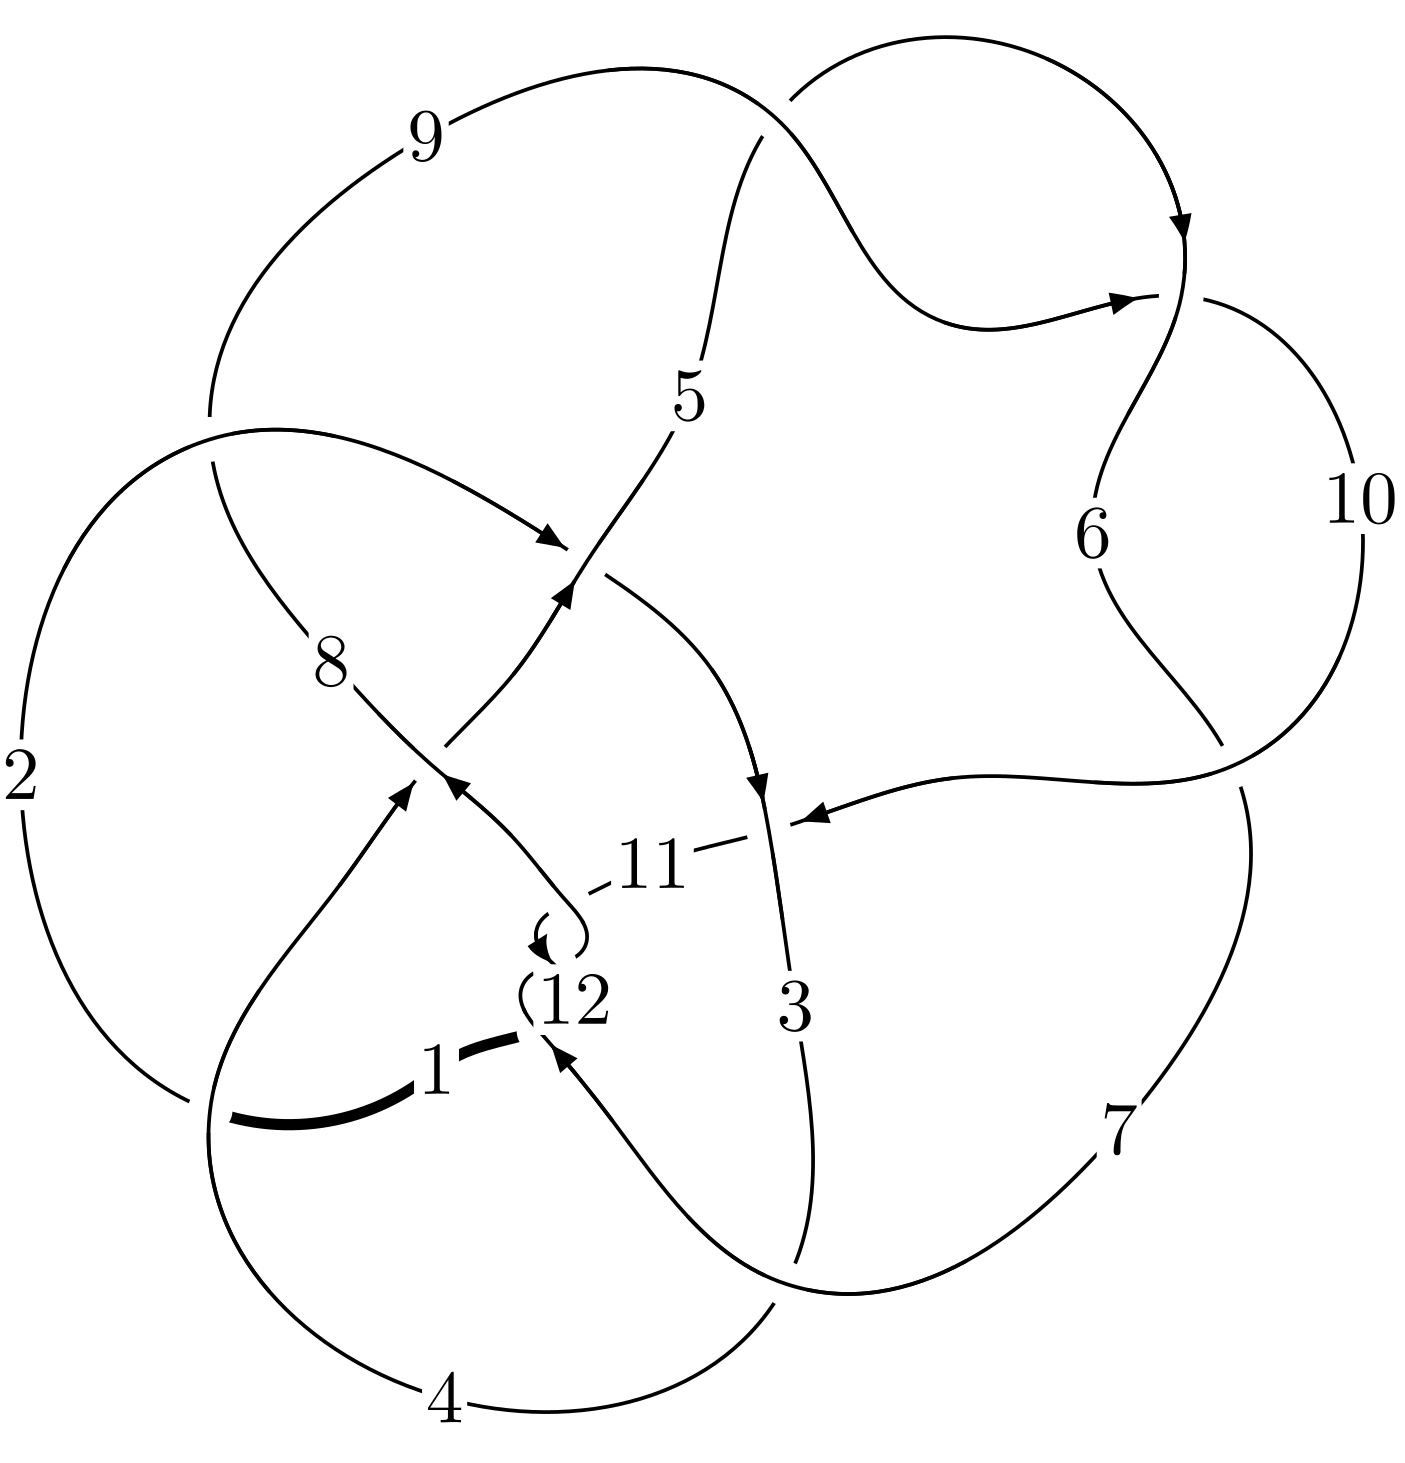
\includegraphics[width=112pt]{../../../GIT/diagram.site/Diagrams/png/2775_12n_0686.png}\\
\ \ \ A knot diagram\footnotemark}&
\allowdisplaybreaks
\textbf{Linearized knot diagam} \\
\cline{2-2}
 &
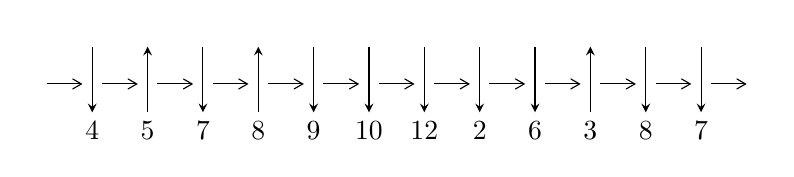
\begin{tikzpicture}[x=20pt, y=17pt]
	% nodes
	\node (C0) at (0, 0) {};
	\node (C1) at (1, 0) {};
	\node (C1U) at (1, +1) {};
	\node (C1D) at (1, -1) {4};

	\node (C2) at (2, 0) {};
	\node (C2U) at (2, +1) {};
	\node (C2D) at (2, -1) {5};

	\node (C3) at (3, 0) {};
	\node (C3U) at (3, +1) {};
	\node (C3D) at (3, -1) {7};

	\node (C4) at (4, 0) {};
	\node (C4U) at (4, +1) {};
	\node (C4D) at (4, -1) {8};

	\node (C5) at (5, 0) {};
	\node (C5U) at (5, +1) {};
	\node (C5D) at (5, -1) {9};

	\node (C6) at (6, 0) {};
	\node (C6U) at (6, +1) {};
	\node (C6D) at (6, -1) {10};

	\node (C7) at (7, 0) {};
	\node (C7U) at (7, +1) {};
	\node (C7D) at (7, -1) {12};

	\node (C8) at (8, 0) {};
	\node (C8U) at (8, +1) {};
	\node (C8D) at (8, -1) {2};

	\node (C9) at (9, 0) {};
	\node (C9U) at (9, +1) {};
	\node (C9D) at (9, -1) {6};

	\node (C10) at (10, 0) {};
	\node (C10U) at (10, +1) {};
	\node (C10D) at (10, -1) {3};

	\node (C11) at (11, 0) {};
	\node (C11U) at (11, +1) {};
	\node (C11D) at (11, -1) {8};

	\node (C12) at (12, 0) {};
	\node (C12U) at (12, +1) {};
	\node (C12D) at (12, -1) {7};
	\node (C13) at (13, 0) {};

	% arrows
	\draw[->,>={angle 60}]
	(C0) edge (C1) (C1) edge (C2) (C2) edge (C3) (C3) edge (C4) (C4) edge (C5) (C5) edge (C6) (C6) edge (C7) (C7) edge (C8) (C8) edge (C9) (C9) edge (C10) (C10) edge (C11) (C11) edge (C12) (C12) edge (C13) ;	\draw[->,>=stealth]
	(C1U) edge (C1D) (C2D) edge (C2U) (C3U) edge (C3D) (C4D) edge (C4U) (C5U) edge (C5D) (C6U) edge (C6D) (C7U) edge (C7D) (C8U) edge (C8D) (C9U) edge (C9D) (C10D) edge (C10U) (C11U) edge (C11D) (C12U) edge (C12D) ;
	\end{tikzpicture} \\
\hhline{~~} \\& 
\textbf{Solving Sequence} \\ \cline{2-2} 
 &
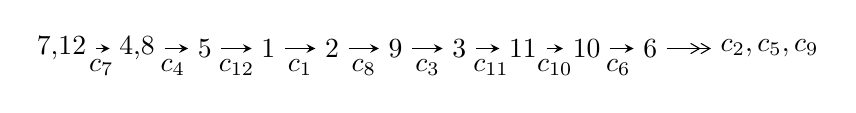
\begin{tikzpicture}[x=23pt, y=7pt]
	% node
	\node (A0) at (-1/8, 0) {7,12};
	\node (A1) at (17/16, 0) {4,8};
	\node (A2) at (17/8, 0) {5};
	\node (A3) at (25/8, 0) {1};
	\node (A4) at (33/8, 0) {2};
	\node (A5) at (41/8, 0) {9};
	\node (A6) at (49/8, 0) {3};
	\node (A7) at (57/8, 0) {11};
	\node (A8) at (65/8, 0) {10};
	\node (A9) at (73/8, 0) {6};
	\node (C1) at (1/2, -1) {$c_{7}$};
	\node (C2) at (13/8, -1) {$c_{4}$};
	\node (C3) at (21/8, -1) {$c_{12}$};
	\node (C4) at (29/8, -1) {$c_{1}$};
	\node (C5) at (37/8, -1) {$c_{8}$};
	\node (C6) at (45/8, -1) {$c_{3}$};
	\node (C7) at (53/8, -1) {$c_{11}$};
	\node (C8) at (61/8, -1) {$c_{10}$};
	\node (C9) at (69/8, -1) {$c_{6}$};
	\node (A10) at (11, 0) {$c_{2},c_{5},c_{9}$};

	% edge
	\draw[->,>=stealth]	
	(A0) edge (A1) (A1) edge (A2) (A2) edge (A3) (A3) edge (A4) (A4) edge (A5) (A5) edge (A6) (A6) edge (A7) (A7) edge (A8) (A8) edge (A9) ;
	\draw[->>,>={angle 60}]	
	(A9) edge (A10);
\end{tikzpicture} \\ 

\end{tabular} \\

\footnotetext{
The image of knot diagram is generated by the software ``\textbf{Draw programme}" developed by Andrew Bartholomew(\url{http://www.layer8.co.uk/maths/draw/index.htm\#Running-draw}), where we modified some parts for our purpose(\url{https://github.com/CATsTAILs/LinksPainter}).
}\phantom \\ \newline 
\centering \textbf{Ideals for irreducible components\footnotemark of $X_{\text{par}}$} 
 
\begin{align*}
I^u_{1}&=\langle 
-2.69505\times10^{130} u^{65}+2.15148\times10^{129} u^{64}+\cdots+2.43963\times10^{130} b-1.45063\times10^{131},\\
\phantom{I^u_{1}}&\phantom{= \langle  }-8.57548\times10^{130} u^{65}+3.16614\times10^{129} u^{64}+\cdots+2.43963\times10^{130} a-6.80613\times10^{131},\\
\phantom{I^u_{1}}&\phantom{= \langle  }u^{66}+8 u^{64}+\cdots+14 u+1\rangle \\
I^u_{2}&=\langle 
- u^{17}- u^{16}+\cdots+b-7 u,\;244 u^{17}+447 u^{16}+\cdots+19 a+657,\;u^{18}+u^{17}+\cdots+8 u^2+1\rangle \\
\\
\end{align*}
\raggedright * 2 irreducible components of $\dim_{\mathbb{C}}=0$, with total 84 representations.\\
\footnotetext{All coefficients of polynomials are rational numbers. But the coefficients are sometimes approximated in decimal forms when there is not enough margin.}
\newpage
\renewcommand{\arraystretch}{1}
\centering \section*{I. $I^u_{1}= \langle -2.70\times10^{130} u^{65}+2.15\times10^{129} u^{64}+\cdots+2.44\times10^{130} b-1.45\times10^{131},\;-8.58\times10^{130} u^{65}+3.17\times10^{129} u^{64}+\cdots+2.44\times10^{130} a-6.81\times10^{131},\;u^{66}+8 u^{64}+\cdots+14 u+1 \rangle$}
\flushleft \textbf{(i) Arc colorings}\\
\begin{tabular}{m{7pt} m{180pt} m{7pt} m{180pt} }
\flushright $a_{7}=$&$\begin{pmatrix}1\\0\end{pmatrix}$ \\
\flushright $a_{12}=$&$\begin{pmatrix}0\\u\end{pmatrix}$ \\
\flushright $a_{4}=$&$\begin{pmatrix}3.51508 u^{65}-0.129779 u^{64}+\cdots+210.106 u+27.8982\\1.10470 u^{65}-0.0881890 u^{64}+\cdots+55.7119 u+5.94611\end{pmatrix}$ \\
\flushright $a_{8}=$&$\begin{pmatrix}1\\u^2\end{pmatrix}$ \\
\flushright $a_{5}=$&$\begin{pmatrix}4.56038 u^{65}-0.0374882 u^{64}+\cdots+267.516 u+33.7146\\1.04992 u^{65}-0.150384 u^{64}+\cdots+53.3745 u+5.85382\end{pmatrix}$ \\
\flushright $a_{1}=$&$\begin{pmatrix}- u\\u\end{pmatrix}$ \\
\flushright $a_{2}=$&$\begin{pmatrix}7.93049 u^{65}-1.14259 u^{64}+\cdots+401.649 u+50.8636\\1.21958 u^{65}-0.156828 u^{64}+\cdots+62.7169 u+7.17179\end{pmatrix}$ \\
\flushright $a_{9}=$&$\begin{pmatrix}11.2952 u^{65}-2.21571 u^{64}+\cdots+527.820 u+67.7880\\0.727751 u^{65}-0.0696228 u^{64}+\cdots+51.3476 u+6.91232\end{pmatrix}$ \\
\flushright $a_{3}=$&$\begin{pmatrix}4.61977 u^{65}-0.217968 u^{64}+\cdots+265.817 u+33.8443\\1.10470 u^{65}-0.0881890 u^{64}+\cdots+55.7119 u+5.94611\end{pmatrix}$ \\
\flushright $a_{11}=$&$\begin{pmatrix}u\\u^3+u\end{pmatrix}$ \\
\flushright $a_{10}=$&$\begin{pmatrix}8.15717 u^{65}-1.17920 u^{64}+\cdots+412.691 u+52.1630\\1.24237 u^{65}-0.0782801 u^{64}+\cdots+63.4671 u+7.14796\end{pmatrix}$ \\
\flushright $a_{6}=$&$\begin{pmatrix}-13.9731 u^{65}+2.50512 u^{64}+\cdots-652.317 u-80.5461\\-1.33472 u^{65}+0.329465 u^{64}+\cdots-50.4358 u-6.86127\end{pmatrix}$\\&\end{tabular}
\flushleft \textbf{(ii) Obstruction class $= -1$}\\~\\
\flushleft \textbf{(iii) Cusp Shapes $= 0.613469 u^{65}+0.240964 u^{64}+\cdots+17.8117 u-7.54006$}\\~\\
\newpage\renewcommand{\arraystretch}{1}
\flushleft \textbf{(iv) u-Polynomials at the component}\newline \\
\begin{tabular}{m{50pt}|m{274pt}}
Crossings & \hspace{64pt}u-Polynomials at each crossing \\
\hline $$\begin{aligned}c_{1}\end{aligned}$$&$\begin{aligned}
&u^{66}+6 u^{65}+\cdots+5840 u+651
\end{aligned}$\\
\hline $$\begin{aligned}c_{2}\end{aligned}$$&$\begin{aligned}
&u^{66}+8 u^{65}+\cdots+244 u-37
\end{aligned}$\\
\hline $$\begin{aligned}c_{3}\end{aligned}$$&$\begin{aligned}
&u^{66}-34 u^{64}+\cdots-1660 u-803
\end{aligned}$\\
\hline $$\begin{aligned}c_{4}\end{aligned}$$&$\begin{aligned}
&u^{66}+8 u^{64}+\cdots+2550 u-731
\end{aligned}$\\
\hline $$\begin{aligned}c_{5},c_{6},c_{9}\end{aligned}$$&$\begin{aligned}
&u^{66}+u^{65}+\cdots+14 u-3
\end{aligned}$\\
\hline $$\begin{aligned}c_{7},c_{11},c_{12}\end{aligned}$$&$\begin{aligned}
&u^{66}+8 u^{64}+\cdots+14 u+1
\end{aligned}$\\
\hline $$\begin{aligned}c_{8}\end{aligned}$$&$\begin{aligned}
&u^{66}+u^{65}+\cdots-979 u-167
\end{aligned}$\\
\hline $$\begin{aligned}c_{10}\end{aligned}$$&$\begin{aligned}
&u^{66}+27 u^{64}+\cdots-2100877 u+215861
\end{aligned}$\\
\hline
\end{tabular}\\~\\
\newpage\renewcommand{\arraystretch}{1}
\flushleft \textbf{(v) Riley Polynomials at the component}\newline \\
\begin{tabular}{m{50pt}|m{274pt}}
Crossings & \hspace{64pt}Riley Polynomials at each crossing \\
\hline $$\begin{aligned}c_{1}\end{aligned}$$&$\begin{aligned}
&y^{66}-70 y^{65}+\cdots-19635172 y+423801
\end{aligned}$\\
\hline $$\begin{aligned}c_{2}\end{aligned}$$&$\begin{aligned}
&y^{66}+18 y^{65}+\cdots-28826 y+1369
\end{aligned}$\\
\hline $$\begin{aligned}c_{3}\end{aligned}$$&$\begin{aligned}
&y^{66}-68 y^{65}+\cdots+49426552 y+644809
\end{aligned}$\\
\hline $$\begin{aligned}c_{4}\end{aligned}$$&$\begin{aligned}
&y^{66}+16 y^{65}+\cdots+19981630 y+534361
\end{aligned}$\\
\hline $$\begin{aligned}c_{5},c_{6},c_{9}\end{aligned}$$&$\begin{aligned}
&y^{66}-71 y^{65}+\cdots-304 y+9
\end{aligned}$\\
\hline $$\begin{aligned}c_{7},c_{11},c_{12}\end{aligned}$$&$\begin{aligned}
&y^{66}+16 y^{65}+\cdots-28 y+1
\end{aligned}$\\
\hline $$\begin{aligned}c_{8}\end{aligned}$$&$\begin{aligned}
&y^{66}-17 y^{65}+\cdots-794781 y+27889
\end{aligned}$\\
\hline $$\begin{aligned}c_{10}\end{aligned}$$&$\begin{aligned}
&y^{66}+54 y^{65}+\cdots-373655164727 y+46595971321
\end{aligned}$\\
\hline
\end{tabular}\\~\\
\newpage\flushleft \textbf{(vi) Complex Volumes and Cusp Shapes}
$$\begin{array}{c|c|c}  
\text{Solutions to }I^u_{1}& \I (\text{vol} + \sqrt{-1}CS) & \text{Cusp shape}\\
 \hline 
\begin{aligned}
u &= \phantom{-}0.381480 + 0.902641 I \\
a &= -0.495217 - 0.818731 I \\
b &= \phantom{-}0.252778 + 0.945202 I\end{aligned}
 & -4.89349 - 2.13130 I & -7.50430 + 3.71654 I \\ \hline\begin{aligned}
u &= \phantom{-}0.381480 - 0.902641 I \\
a &= -0.495217 + 0.818731 I \\
b &= \phantom{-}0.252778 - 0.945202 I\end{aligned}
 & -4.89349 + 2.13130 I & -7.50430 - 3.71654 I \\ \hline\begin{aligned}
u &= -0.038908 + 0.939745 I \\
a &= -0.275001 - 0.321868 I \\
b &= -0.871697 + 0.971052 I\end{aligned}
 & -3.77402 - 3.72825 I & -5.26113 + 2.10644 I \\ \hline\begin{aligned}
u &= -0.038908 - 0.939745 I \\
a &= -0.275001 + 0.321868 I \\
b &= -0.871697 - 0.971052 I\end{aligned}
 & -3.77402 + 3.72825 I & -5.26113 - 2.10644 I \\ \hline\begin{aligned}
u &= \phantom{-}0.905831 + 0.018069 I \\
a &= -0.533383 + 0.894315 I \\
b &= \phantom{-}0.0381606 - 0.1308590 I\end{aligned}
 & -7.85798 + 1.54242 I & -13.03025 - 0.57872 I \\ \hline\begin{aligned}
u &= \phantom{-}0.905831 - 0.018069 I \\
a &= -0.533383 - 0.894315 I \\
b &= \phantom{-}0.0381606 + 0.1308590 I\end{aligned}
 & -7.85798 - 1.54242 I & -13.03025 + 0.57872 I \\ \hline\begin{aligned}
u &= -0.265939 + 0.798350 I \\
a &= \phantom{-}0.838512 - 0.776076 I \\
b &= \phantom{-}0.057693 + 0.475963 I\end{aligned}
 & \phantom{-}1.00311 + 2.04923 I & -3.92564 - 3.61296 I \\ \hline\begin{aligned}
u &= -0.265939 - 0.798350 I \\
a &= \phantom{-}0.838512 + 0.776076 I \\
b &= \phantom{-}0.057693 - 0.475963 I\end{aligned}
 & \phantom{-}1.00311 - 2.04923 I & -3.92564 + 3.61296 I \\ \hline\begin{aligned}
u &= -0.755298 + 0.895200 I \\
a &= -1.00097 + 1.25369 I \\
b &= \phantom{-}1.87437 + 0.23139 I\end{aligned}
 & -11.19350 + 0.70321 I & \phantom{-0.000000 } 0 \\ \hline\begin{aligned}
u &= -0.755298 - 0.895200 I \\
a &= -1.00097 - 1.25369 I \\
b &= \phantom{-}1.87437 - 0.23139 I\end{aligned}
 & -11.19350 - 0.70321 I & \phantom{-0.000000 } 0\\
 \hline 
 \end{array}$$\newpage$$\begin{array}{c|c|c}  
\text{Solutions to }I^u_{1}& \I (\text{vol} + \sqrt{-1}CS) & \text{Cusp shape}\\
 \hline 
\begin{aligned}
u &= -0.496215 + 0.652094 I \\
a &= \phantom{-}0.27441 + 1.70971 I \\
b &= \phantom{-}0.62615 - 1.80443 I\end{aligned}
 & -5.71011 + 7.01316 I & -9.56711 - 9.06601 I \\ \hline\begin{aligned}
u &= -0.496215 - 0.652094 I \\
a &= \phantom{-}0.27441 - 1.70971 I \\
b &= \phantom{-}0.62615 + 1.80443 I\end{aligned}
 & -5.71011 - 7.01316 I & -9.56711 + 9.06601 I \\ \hline\begin{aligned}
u &= \phantom{-}0.830499 + 0.849156 I \\
a &= \phantom{-}0.256829 + 1.321510 I \\
b &= -1.65652 - 0.66579 I\end{aligned}
 & -4.73481 - 4.19817 I & \phantom{-0.000000 } 0 \\ \hline\begin{aligned}
u &= \phantom{-}0.830499 - 0.849156 I \\
a &= \phantom{-}0.256829 - 1.321510 I \\
b &= -1.65652 + 0.66579 I\end{aligned}
 & -4.73481 + 4.19817 I & \phantom{-0.000000 } 0 \\ \hline\begin{aligned}
u &= -0.792820 + 0.887815 I \\
a &= -0.33108 + 1.50593 I \\
b &= \phantom{-}2.02793 - 0.81025 I\end{aligned}
 & -11.23670 + 5.15790 I & \phantom{-0.000000 } 0 \\ \hline\begin{aligned}
u &= -0.792820 - 0.887815 I \\
a &= -0.33108 - 1.50593 I \\
b &= \phantom{-}2.02793 + 0.81025 I\end{aligned}
 & -11.23670 - 5.15790 I & \phantom{-0.000000 } 0 \\ \hline\begin{aligned}
u &= -0.185557 + 1.202860 I \\
a &= \phantom{-}0.628073 - 1.140700 I \\
b &= -0.424674 + 0.578911 I\end{aligned}
 & \phantom{-}2.05717 + 2.26630 I & \phantom{-0.000000 } 0 \\ \hline\begin{aligned}
u &= -0.185557 - 1.202860 I \\
a &= \phantom{-}0.628073 + 1.140700 I \\
b &= -0.424674 - 0.578911 I\end{aligned}
 & \phantom{-}2.05717 - 2.26630 I & \phantom{-0.000000 } 0 \\ \hline\begin{aligned}
u &= -0.166375 + 0.760046 I \\
a &= -2.11546 - 1.78936 I \\
b &= \phantom{-}0.611150 + 1.095880 I\end{aligned}
 & -5.12370 - 4.24500 I & -6.05961 - 1.11595 I \\ \hline\begin{aligned}
u &= -0.166375 - 0.760046 I \\
a &= -2.11546 + 1.78936 I \\
b &= \phantom{-}0.611150 - 1.095880 I\end{aligned}
 & -5.12370 + 4.24500 I & -6.05961 + 1.11595 I\\
 \hline 
 \end{array}$$\newpage$$\begin{array}{c|c|c}  
\text{Solutions to }I^u_{1}& \I (\text{vol} + \sqrt{-1}CS) & \text{Cusp shape}\\
 \hline 
\begin{aligned}
u &= \phantom{-}0.017260 + 0.775267 I \\
a &= \phantom{-}0.72199 - 1.86824 I \\
b &= -0.239640 + 0.901747 I\end{aligned}
 & \phantom{-}1.81981 + 1.76274 I & -0.73012 - 3.27359 I \\ \hline\begin{aligned}
u &= \phantom{-}0.017260 - 0.775267 I \\
a &= \phantom{-}0.72199 + 1.86824 I \\
b &= -0.239640 - 0.901747 I\end{aligned}
 & \phantom{-}1.81981 - 1.76274 I & -0.73012 + 3.27359 I \\ \hline\begin{aligned}
u &= \phantom{-}0.779311 + 0.979842 I \\
a &= \phantom{-}0.771946 + 0.959390 I \\
b &= -1.60829 + 0.02335 I\end{aligned}
 & -4.32456 - 1.86631 I & \phantom{-0.000000 } 0 \\ \hline\begin{aligned}
u &= \phantom{-}0.779311 - 0.979842 I \\
a &= \phantom{-}0.771946 - 0.959390 I \\
b &= -1.60829 - 0.02335 I\end{aligned}
 & -4.32456 + 1.86631 I & \phantom{-0.000000 } 0 \\ \hline\begin{aligned}
u &= -1.020010 + 0.782197 I \\
a &= -0.059578 + 1.004880 I \\
b &= \phantom{-}1.247920 - 0.361242 I\end{aligned}
 & -4.77746 + 2.77204 I & \phantom{-0.000000 } 0 \\ \hline\begin{aligned}
u &= -1.020010 - 0.782197 I \\
a &= -0.059578 - 1.004880 I \\
b &= \phantom{-}1.247920 + 0.361242 I\end{aligned}
 & -4.77746 - 2.77204 I & \phantom{-0.000000 } 0 \\ \hline\begin{aligned}
u &= \phantom{-}1.005160 + 0.805635 I \\
a &= -0.761996 - 0.469288 I \\
b &= \phantom{-}1.85270 + 0.11551 I\end{aligned}
 & -12.76450 - 5.71162 I & \phantom{-0.000000 } 0 \\ \hline\begin{aligned}
u &= \phantom{-}1.005160 - 0.805635 I \\
a &= -0.761996 + 0.469288 I \\
b &= \phantom{-}1.85270 - 0.11551 I\end{aligned}
 & -12.76450 + 5.71162 I & \phantom{-0.000000 } 0 \\ \hline\begin{aligned}
u &= \phantom{-}0.021107 + 0.705377 I \\
a &= \phantom{-}0.578182 + 0.067715 I \\
b &= \phantom{-}0.834319 + 0.472388 I\end{aligned}
 & \phantom{-}1.57907 + 2.38485 I & -0.324197 - 0.690209 I \\ \hline\begin{aligned}
u &= \phantom{-}0.021107 - 0.705377 I \\
a &= \phantom{-}0.578182 - 0.067715 I \\
b &= \phantom{-}0.834319 - 0.472388 I\end{aligned}
 & \phantom{-}1.57907 - 2.38485 I & -0.324197 + 0.690209 I\\
 \hline 
 \end{array}$$\newpage$$\begin{array}{c|c|c}  
\text{Solutions to }I^u_{1}& \I (\text{vol} + \sqrt{-1}CS) & \text{Cusp shape}\\
 \hline 
\begin{aligned}
u &= \phantom{-}0.490966 + 0.475053 I \\
a &= -0.55254 + 1.62553 I \\
b &= -0.09615 - 1.50670 I\end{aligned}
 & \phantom{-}0.16917 - 3.95160 I & -7.93720 + 9.53197 I \\ \hline\begin{aligned}
u &= \phantom{-}0.490966 - 0.475053 I \\
a &= -0.55254 - 1.62553 I \\
b &= -0.09615 + 1.50670 I\end{aligned}
 & \phantom{-}0.16917 + 3.95160 I & -7.93720 - 9.53197 I \\ \hline\begin{aligned}
u &= \phantom{-}0.379973 + 0.551049 I \\
a &= -1.78771 - 0.92141 I \\
b &= -0.300972 - 0.209570 I\end{aligned}
 & \phantom{-}0.75753 - 4.12116 I & -7.35035 + 12.02767 I \\ \hline\begin{aligned}
u &= \phantom{-}0.379973 - 0.551049 I \\
a &= -1.78771 + 0.92141 I \\
b &= -0.300972 + 0.209570 I\end{aligned}
 & \phantom{-}0.75753 + 4.12116 I & -7.35035 - 12.02767 I \\ \hline\begin{aligned}
u &= -1.064810 + 0.801331 I \\
a &= \phantom{-}0.792009 - 0.579040 I \\
b &= -1.72587 + 0.09376 I\end{aligned}
 & -5.93827 + 1.09172 I & \phantom{-0.000000 } 0 \\ \hline\begin{aligned}
u &= -1.064810 - 0.801331 I \\
a &= \phantom{-}0.792009 + 0.579040 I \\
b &= -1.72587 - 0.09376 I\end{aligned}
 & -5.93827 - 1.09172 I & \phantom{-0.000000 } 0 \\ \hline\begin{aligned}
u &= -0.143019 + 1.344970 I \\
a &= -0.473522 - 0.509487 I \\
b &= \phantom{-}0.417362 + 0.247824 I\end{aligned}
 & \phantom{-}3.24630 + 2.81207 I & \phantom{-0.000000 } 0 \\ \hline\begin{aligned}
u &= -0.143019 - 1.344970 I \\
a &= -0.473522 + 0.509487 I \\
b &= \phantom{-}0.417362 - 0.247824 I\end{aligned}
 & \phantom{-}3.24630 - 2.81207 I & \phantom{-0.000000 } 0 \\ \hline\begin{aligned}
u &= \phantom{-}1.089300 + 0.810624 I \\
a &= -0.721178 - 0.626134 I \\
b &= \phantom{-}1.64027 - 0.04042 I\end{aligned}
 & -6.51348 + 4.48861 I & \phantom{-0.000000 } 0 \\ \hline\begin{aligned}
u &= \phantom{-}1.089300 - 0.810624 I \\
a &= -0.721178 + 0.626134 I \\
b &= \phantom{-}1.64027 + 0.04042 I\end{aligned}
 & -6.51348 - 4.48861 I & \phantom{-0.000000 } 0\\
 \hline 
 \end{array}$$\newpage$$\begin{array}{c|c|c}  
\text{Solutions to }I^u_{1}& \I (\text{vol} + \sqrt{-1}CS) & \text{Cusp shape}\\
 \hline 
\begin{aligned}
u &= -0.474413 + 0.430132 I \\
a &= \phantom{-}2.22892 - 1.47522 I \\
b &= \phantom{-}0.398954 - 0.549454 I\end{aligned}
 & -5.98479 + 5.90839 I & -10.77299 - 9.08116 I \\ \hline\begin{aligned}
u &= -0.474413 - 0.430132 I \\
a &= \phantom{-}2.22892 + 1.47522 I \\
b &= \phantom{-}0.398954 + 0.549454 I\end{aligned}
 & -5.98479 - 5.90839 I & -10.77299 + 9.08116 I \\ \hline\begin{aligned}
u &= -1.117140 + 0.824420 I \\
a &= \phantom{-}0.676641 - 0.619494 I \\
b &= -1.66630 - 0.17442 I\end{aligned}
 & -13.8794 - 8.3029 I & \phantom{-0.000000 } 0 \\ \hline\begin{aligned}
u &= -1.117140 - 0.824420 I \\
a &= \phantom{-}0.676641 + 0.619494 I \\
b &= -1.66630 + 0.17442 I\end{aligned}
 & -13.8794 + 8.3029 I & \phantom{-0.000000 } 0 \\ \hline\begin{aligned}
u &= \phantom{-}0.868320 + 1.114680 I \\
a &= -0.75239 - 1.40142 I \\
b &= \phantom{-}1.42271 + 0.41666 I\end{aligned}
 & -11.78330 - 1.19681 I & \phantom{-0.000000 } 0 \\ \hline\begin{aligned}
u &= \phantom{-}0.868320 - 1.114680 I \\
a &= -0.75239 + 1.40142 I \\
b &= \phantom{-}1.42271 - 0.41666 I\end{aligned}
 & -11.78330 + 1.19681 I & \phantom{-0.000000 } 0 \\ \hline\begin{aligned}
u &= \phantom{-}1.20197 + 0.75106 I \\
a &= -0.035347 + 0.853586 I \\
b &= -1.196160 - 0.140651 I\end{aligned}
 & -11.31340 - 2.25996 I & \phantom{-0.000000 } 0 \\ \hline\begin{aligned}
u &= \phantom{-}1.20197 - 0.75106 I \\
a &= -0.035347 - 0.853586 I \\
b &= -1.196160 + 0.140651 I\end{aligned}
 & -11.31340 + 2.25996 I & \phantom{-0.000000 } 0 \\ \hline\begin{aligned}
u &= -0.91284 + 1.08691 I \\
a &= -0.446199 + 0.740868 I \\
b &= \phantom{-}1.41565 - 0.16249 I\end{aligned}
 & -3.84346 + 4.28579 I & \phantom{-0.000000 } 0 \\ \hline\begin{aligned}
u &= -0.91284 - 1.08691 I \\
a &= -0.446199 - 0.740868 I \\
b &= \phantom{-}1.41565 + 0.16249 I\end{aligned}
 & -3.84346 - 4.28579 I & \phantom{-0.000000 } 0\\
 \hline 
 \end{array}$$\newpage$$\begin{array}{c|c|c}  
\text{Solutions to }I^u_{1}& \I (\text{vol} + \sqrt{-1}CS) & \text{Cusp shape}\\
 \hline 
\begin{aligned}
u &= \phantom{-}0.91205 + 1.11570 I \\
a &= -0.63727 - 1.31272 I \\
b &= \phantom{-}1.67828 + 0.62567 I\end{aligned}
 & -5.52111 - 11.73990 I & \phantom{-0.000000 } 0 \\ \hline\begin{aligned}
u &= \phantom{-}0.91205 - 1.11570 I \\
a &= -0.63727 + 1.31272 I \\
b &= \phantom{-}1.67828 - 0.62567 I\end{aligned}
 & -5.52111 + 11.73990 I & \phantom{-0.000000 } 0 \\ \hline\begin{aligned}
u &= -0.91053 + 1.11720 I \\
a &= \phantom{-}0.70943 - 1.31981 I \\
b &= -1.55420 + 0.57473 I\end{aligned}
 & -4.93579 + 6.09434 I & \phantom{-0.000000 } 0 \\ \hline\begin{aligned}
u &= -0.91053 - 1.11720 I \\
a &= \phantom{-}0.70943 + 1.31981 I \\
b &= -1.55420 - 0.57473 I\end{aligned}
 & -4.93579 - 6.09434 I & \phantom{-0.000000 } 0 \\ \hline\begin{aligned}
u &= -0.91964 + 1.12282 I \\
a &= \phantom{-}0.59423 - 1.33466 I \\
b &= -1.79214 + 0.62953 I\end{aligned}
 & -12.8813 + 15.6604 I & \phantom{-0.000000 } 0 \\ \hline\begin{aligned}
u &= -0.91964 - 1.12282 I \\
a &= \phantom{-}0.59423 + 1.33466 I \\
b &= -1.79214 - 0.62953 I\end{aligned}
 & -12.8813 - 15.6604 I & \phantom{-0.000000 } 0 \\ \hline\begin{aligned}
u &= -0.514106 + 0.183956 I \\
a &= \phantom{-}0.91070 + 1.13917 I \\
b &= -0.429112 - 0.679047 I\end{aligned}
 & -0.992824 + 0.084224 I & -11.71855 + 1.75099 I \\ \hline\begin{aligned}
u &= -0.514106 - 0.183956 I \\
a &= \phantom{-}0.91070 - 1.13917 I \\
b &= -0.429112 + 0.679047 I\end{aligned}
 & -0.992824 - 0.084224 I & -11.71855 - 1.75099 I \\ \hline\begin{aligned}
u &= \phantom{-}0.32591 + 1.42708 I \\
a &= \phantom{-}0.480076 - 0.162455 I \\
b &= -0.612916 - 0.001301 I\end{aligned}
 & -2.95398 - 6.38488 I & \phantom{-0.000000 } 0 \\ \hline\begin{aligned}
u &= \phantom{-}0.32591 - 1.42708 I \\
a &= \phantom{-}0.480076 + 0.162455 I \\
b &= -0.612916 + 0.001301 I\end{aligned}
 & -2.95398 + 6.38488 I & \phantom{-0.000000 } 0\\
 \hline 
 \end{array}$$\newpage$$\begin{array}{c|c|c}  
\text{Solutions to }I^u_{1}& \I (\text{vol} + \sqrt{-1}CS) & \text{Cusp shape}\\
 \hline 
\begin{aligned}
u &= \phantom{-}1.04603 + 1.17919 I \\
a &= \phantom{-}0.290516 + 0.627195 I \\
b &= -1.387930 - 0.223326 I\end{aligned}
 & -10.02500 - 5.74966 I & \phantom{-0.000000 } 0 \\ \hline\begin{aligned}
u &= \phantom{-}1.04603 - 1.17919 I \\
a &= \phantom{-}0.290516 - 0.627195 I \\
b &= -1.387930 + 0.223326 I\end{aligned}
 & -10.02500 + 5.74966 I & \phantom{-0.000000 } 0 \\ \hline\begin{aligned}
u &= -0.228442 + 0.312802 I \\
a &= \phantom{-}0.53438 + 1.55461 I \\
b &= -1.109960 - 0.068072 I\end{aligned}
 & -0.710026 + 0.001156 I & -6.94437 - 0.21585 I \\ \hline\begin{aligned}
u &= -0.228442 - 0.312802 I \\
a &= \phantom{-}0.53438 - 1.55461 I \\
b &= -1.109960 + 0.068072 I\end{aligned}
 & -0.710026 - 0.001156 I & -6.94437 + 0.21585 I \\ \hline\begin{aligned}
u &= -0.332795\phantom{ +0.000000I} \\
a &= \phantom{-}1.34321\phantom{ +0.000000I} \\
b &= -0.576763\phantom{ +0.000000I}\end{aligned}
 & -0.861436\phantom{ +0.000000I} & -11.4550\phantom{ +0.000000I} \\ \hline\begin{aligned}
u &= -0.165446\phantom{ +0.000000I} \\
a &= \phantom{-}9.04077\phantom{ +0.000000I} \\
b &= \phantom{-}1.12903\phantom{ +0.000000I}\end{aligned}
 & -8.63556\phantom{ +0.000000I} & -9.01670\phantom{ +0.000000I}\\
 \hline 
 \end{array}$$\newpage\newpage\renewcommand{\arraystretch}{1}
\centering \section*{II. $I^u_{2}= \langle - u^{17}- u^{16}+\cdots+b-7 u,\;244 u^{17}+447 u^{16}+\cdots+19 a+657,\;u^{18}+u^{17}+\cdots+8 u^2+1 \rangle$}
\flushleft \textbf{(i) Arc colorings}\\
\begin{tabular}{m{7pt} m{180pt} m{7pt} m{180pt} }
\flushright $a_{7}=$&$\begin{pmatrix}1\\0\end{pmatrix}$ \\
\flushright $a_{12}=$&$\begin{pmatrix}0\\u\end{pmatrix}$ \\
\flushright $a_{4}=$&$\begin{pmatrix}-12.8421 u^{17}-23.5263 u^{16}+\cdots-27.7895 u-34.5789\\u^{17}+u^{16}+\cdots+27 u^3+7 u\end{pmatrix}$ \\
\flushright $a_{8}=$&$\begin{pmatrix}1\\u^2\end{pmatrix}$ \\
\flushright $a_{5}=$&$\begin{pmatrix}-17.4737 u^{17}-31.4211 u^{16}+\cdots-33.6316 u-45.2632\\3.47368 u^{17}+4.42105 u^{16}+\cdots+11.6316 u+3.26316\end{pmatrix}$ \\
\flushright $a_{1}=$&$\begin{pmatrix}- u\\u\end{pmatrix}$ \\
\flushright $a_{2}=$&$\begin{pmatrix}-4.89474 u^{17}+8.31579 u^{16}+\cdots-35.5263 u+38.9474\\-6.21053 u^{17}-13.6316 u^{16}+\cdots-7.94737 u-23.8947\end{pmatrix}$ \\
\flushright $a_{9}=$&$\begin{pmatrix}4.68421 u^{17}-11.9474 u^{16}+\cdots+27.5789 u-48.8421\\8.10526 u^{17}+9.31579 u^{16}+\cdots+22.4737 u+7.94737\end{pmatrix}$ \\
\flushright $a_{3}=$&$\begin{pmatrix}-11.8421 u^{17}-22.5263 u^{16}+\cdots-20.7895 u-34.5789\\u^{17}+u^{16}+\cdots+27 u^3+7 u\end{pmatrix}$ \\
\flushright $a_{11}=$&$\begin{pmatrix}u\\u^3+u\end{pmatrix}$ \\
\flushright $a_{10}=$&$\begin{pmatrix}-2.31579 u^{17}+9.05263 u^{16}+\cdots-22.4211 u+33.1579\\-4.05263 u^{17}-9.15789 u^{16}+\cdots-7.73684 u-16.4737\end{pmatrix}$ \\
\flushright $a_{6}=$&$\begin{pmatrix}-8.36842 u^{17}+3.89474 u^{16}+\cdots-37.1579 u+36.6842\\-9.52632 u^{17}-13.5789 u^{16}+\cdots-21.3684 u-15.7368\end{pmatrix}$\\&\end{tabular}
\flushleft \textbf{(ii) Obstruction class $= 1$}\\~\\
\flushleft \textbf{(iii) Cusp Shapes $= 49 u^{17}+9 u^{16}+240 u^{15}+9 u^{14}+621 u^{13}-98 u^{12}+1237 u^{11}-361 u^{10}+1867 u^9-760 u^8+1897 u^7-1242 u^6+1412 u^5-1233 u^4+809 u^3-508 u^2+170 u-89$}\\~\\
\newpage\renewcommand{\arraystretch}{1}
\flushleft \textbf{(iv) u-Polynomials at the component}\newline \\
\begin{tabular}{m{50pt}|m{274pt}}
Crossings & \hspace{64pt}u-Polynomials at each crossing \\
\hline $$\begin{aligned}c_{1}\end{aligned}$$&$\begin{aligned}
&u^{18}-13 u^{17}+\cdots-88 u+11
\end{aligned}$\\
\hline $$\begin{aligned}c_{2}\end{aligned}$$&$\begin{aligned}
&u^{18}+5 u^{17}+\cdots+2 u+1
\end{aligned}$\\
\hline $$\begin{aligned}c_{3}\end{aligned}$$&$\begin{aligned}
&u^{18}+u^{17}+\cdots+6 u^2+1
\end{aligned}$\\
\hline $$\begin{aligned}c_{4}\end{aligned}$$&$\begin{aligned}
&u^{18}- u^{17}+\cdots+u^2+1
\end{aligned}$\\
\hline $$\begin{aligned}c_{5},c_{6}\end{aligned}$$&$\begin{aligned}
&u^{18}-10 u^{16}+\cdots-2 u+1
\end{aligned}$\\
\hline $$\begin{aligned}c_{7}\end{aligned}$$&$\begin{aligned}
&u^{18}+u^{17}+\cdots+8 u^2+1
\end{aligned}$\\
\hline $$\begin{aligned}c_{8}\end{aligned}$$&$\begin{aligned}
&u^{18}+u^{16}+\cdots+u+1
\end{aligned}$\\
\hline $$\begin{aligned}c_{9}\end{aligned}$$&$\begin{aligned}
&u^{18}-10 u^{16}+\cdots+2 u+1
\end{aligned}$\\
\hline $$\begin{aligned}c_{10}\end{aligned}$$&$\begin{aligned}
&u^{18}+3 u^{17}+\cdots-3 u+1
\end{aligned}$\\
\hline $$\begin{aligned}c_{11},c_{12}\end{aligned}$$&$\begin{aligned}
&u^{18}- u^{17}+\cdots+8 u^2+1
\end{aligned}$\\
\hline
\end{tabular}\\~\\
\newpage\renewcommand{\arraystretch}{1}
\flushleft \textbf{(v) Riley Polynomials at the component}\newline \\
\begin{tabular}{m{50pt}|m{274pt}}
Crossings & \hspace{64pt}Riley Polynomials at each crossing \\
\hline $$\begin{aligned}c_{1}\end{aligned}$$&$\begin{aligned}
&y^{18}-7 y^{17}+\cdots+968 y+121
\end{aligned}$\\
\hline $$\begin{aligned}c_{2}\end{aligned}$$&$\begin{aligned}
&y^{18}+y^{17}+\cdots+2 y+1
\end{aligned}$\\
\hline $$\begin{aligned}c_{3}\end{aligned}$$&$\begin{aligned}
&y^{18}-9 y^{17}+\cdots+12 y+1
\end{aligned}$\\
\hline $$\begin{aligned}c_{4}\end{aligned}$$&$\begin{aligned}
&y^{18}-5 y^{17}+\cdots+2 y+1
\end{aligned}$\\
\hline $$\begin{aligned}c_{5},c_{6},c_{9}\end{aligned}$$&$\begin{aligned}
&y^{18}-20 y^{17}+\cdots+16 y+1
\end{aligned}$\\
\hline $$\begin{aligned}c_{7},c_{11},c_{12}\end{aligned}$$&$\begin{aligned}
&y^{18}+11 y^{17}+\cdots+16 y+1
\end{aligned}$\\
\hline $$\begin{aligned}c_{8}\end{aligned}$$&$\begin{aligned}
&y^{18}+2 y^{17}+\cdots-5 y+1
\end{aligned}$\\
\hline $$\begin{aligned}c_{10}\end{aligned}$$&$\begin{aligned}
&y^{18}+13 y^{17}+\cdots-7 y+1
\end{aligned}$\\
\hline
\end{tabular}\\~\\
\newpage\flushleft \textbf{(vi) Complex Volumes and Cusp Shapes}
$$\begin{array}{c|c|c}  
\text{Solutions to }I^u_{2}& \I (\text{vol} + \sqrt{-1}CS) & \text{Cusp shape}\\
 \hline 
\begin{aligned}
u &= -0.804642 + 0.868057 I \\
a &= -0.36882 + 1.48135 I \\
b &= \phantom{-}1.378990 - 0.248447 I\end{aligned}
 & -9.83536 + 1.64758 I & -9.43619 - 2.86445 I \\ \hline\begin{aligned}
u &= -0.804642 - 0.868057 I \\
a &= -0.36882 - 1.48135 I \\
b &= \phantom{-}1.378990 + 0.248447 I\end{aligned}
 & -9.83536 - 1.64758 I & -9.43619 + 2.86445 I \\ \hline\begin{aligned}
u &= \phantom{-}0.044577 + 1.238730 I \\
a &= -0.408391 + 0.683987 I \\
b &= -0.073590 - 0.432493 I\end{aligned}
 & \phantom{-}3.80104 - 3.17945 I & \phantom{-}1.80104 + 7.13521 I \\ \hline\begin{aligned}
u &= \phantom{-}0.044577 - 1.238730 I \\
a &= -0.408391 - 0.683987 I \\
b &= -0.073590 + 0.432493 I\end{aligned}
 & \phantom{-}3.80104 + 3.17945 I & \phantom{-}1.80104 - 7.13521 I \\ \hline\begin{aligned}
u &= \phantom{-}0.264515 + 1.248310 I \\
a &= \phantom{-}0.649266 + 1.187430 I \\
b &= -0.426970 - 0.481643 I\end{aligned}
 & \phantom{-}1.90679 - 1.92588 I & -11.44215 - 7.89971 I \\ \hline\begin{aligned}
u &= \phantom{-}0.264515 - 1.248310 I \\
a &= \phantom{-}0.649266 - 1.187430 I \\
b &= -0.426970 + 0.481643 I\end{aligned}
 & \phantom{-}1.90679 + 1.92588 I & -11.44215 + 7.89971 I \\ \hline\begin{aligned}
u &= \phantom{-}0.925026 + 0.906908 I \\
a &= \phantom{-}0.360696 + 1.026960 I \\
b &= -1.47624 - 0.36649 I\end{aligned}
 & -4.24577 - 3.38226 I & -8.45773 + 3.28670 I \\ \hline\begin{aligned}
u &= \phantom{-}0.925026 - 0.906908 I \\
a &= \phantom{-}0.360696 - 1.026960 I \\
b &= -1.47624 + 0.36649 I\end{aligned}
 & -4.24577 + 3.38226 I & -8.45773 - 3.28670 I \\ \hline\begin{aligned}
u &= -0.238208 + 1.279130 I \\
a &= \phantom{-}0.256462 + 0.472498 I \\
b &= \phantom{-}0.378917 - 0.523548 I\end{aligned}
 & -2.11329 + 6.53754 I & -2.93657 - 5.70476 I \\ \hline\begin{aligned}
u &= -0.238208 - 1.279130 I \\
a &= \phantom{-}0.256462 - 0.472498 I \\
b &= \phantom{-}0.378917 + 0.523548 I\end{aligned}
 & -2.11329 - 6.53754 I & -2.93657 + 5.70476 I\\
 \hline 
 \end{array}$$\newpage$$\begin{array}{c|c|c}  
\text{Solutions to }I^u_{2}& \I (\text{vol} + \sqrt{-1}CS) & \text{Cusp shape}\\
 \hline 
\begin{aligned}
u &= -0.943992 + 0.928790 I \\
a &= -0.161234 + 0.776586 I \\
b &= \phantom{-}1.48226 - 0.39919 I\end{aligned}
 & -9.59239 + 4.85624 I & -9.87202 - 2.24813 I \\ \hline\begin{aligned}
u &= -0.943992 - 0.928790 I \\
a &= -0.161234 - 0.776586 I \\
b &= \phantom{-}1.48226 + 0.39919 I\end{aligned}
 & -9.59239 - 4.85624 I & -9.87202 + 2.24813 I \\ \hline\begin{aligned}
u &= \phantom{-}0.382414 + 0.542277 I \\
a &= \phantom{-}0.290004 - 0.853492 I \\
b &= -1.25094 + 0.68932 I\end{aligned}
 & -0.681831 - 0.856086 I & -6.33441 + 8.31733 I \\ \hline\begin{aligned}
u &= \phantom{-}0.382414 - 0.542277 I \\
a &= \phantom{-}0.290004 + 0.853492 I \\
b &= -1.25094 - 0.68932 I\end{aligned}
 & -0.681831 + 0.856086 I & -6.33441 - 8.31733 I \\ \hline\begin{aligned}
u &= -0.071184 + 0.625824 I \\
a &= \phantom{-}1.41490 - 1.09388 I \\
b &= \phantom{-}0.250613 + 0.951659 I\end{aligned}
 & \phantom{-}1.25984 + 3.18601 I & -2.50556 - 8.38071 I \\ \hline\begin{aligned}
u &= -0.071184 - 0.625824 I \\
a &= \phantom{-}1.41490 + 1.09388 I \\
b &= \phantom{-}0.250613 - 0.951659 I\end{aligned}
 & \phantom{-}1.25984 - 3.18601 I & -2.50556 + 8.38071 I \\ \hline\begin{aligned}
u &= -0.058505 + 0.569575 I \\
a &= -3.03288 - 1.16293 I \\
b &= \phantom{-}0.236963 + 1.167790 I\end{aligned}
 & -5.17305 - 5.14099 I & -6.31641 + 6.34700 I \\ \hline\begin{aligned}
u &= -0.058505 - 0.569575 I \\
a &= -3.03288 + 1.16293 I \\
b &= \phantom{-}0.236963 - 1.167790 I\end{aligned}
 & -5.17305 + 5.14099 I & -6.31641 - 6.34700 I\\
 \hline 
 \end{array}$$\newpage
\newpage\renewcommand{\arraystretch}{1}
\centering \section*{ III. u-Polynomials}
\begin{tabular}{m{50pt}|m{274pt}}
Crossings & \hspace{64pt}u-Polynomials at each crossing \\
\hline $$\begin{aligned}c_{1}\end{aligned}$$&$\begin{aligned}
&(u^{18}-13 u^{17}+\cdots-88 u+11)(u^{66}+6 u^{65}+\cdots+5840 u+651)
\end{aligned}$\\
\hline $$\begin{aligned}c_{2}\end{aligned}$$&$\begin{aligned}
&(u^{18}+5 u^{17}+\cdots+2 u+1)(u^{66}+8 u^{65}+\cdots+244 u-37)
\end{aligned}$\\
\hline $$\begin{aligned}c_{3}\end{aligned}$$&$\begin{aligned}
&(u^{18}+u^{17}+\cdots+6 u^2+1)(u^{66}-34 u^{64}+\cdots-1660 u-803)
\end{aligned}$\\
\hline $$\begin{aligned}c_{4}\end{aligned}$$&$\begin{aligned}
&(u^{18}- u^{17}+\cdots+u^2+1)(u^{66}+8 u^{64}+\cdots+2550 u-731)
\end{aligned}$\\
\hline $$\begin{aligned}c_{5},c_{6}\end{aligned}$$&$\begin{aligned}
&(u^{18}-10 u^{16}+\cdots-2 u+1)(u^{66}+u^{65}+\cdots+14 u-3)
\end{aligned}$\\
\hline $$\begin{aligned}c_{7}\end{aligned}$$&$\begin{aligned}
&(u^{18}+u^{17}+\cdots+8 u^2+1)(u^{66}+8 u^{64}+\cdots+14 u+1)
\end{aligned}$\\
\hline $$\begin{aligned}c_{8}\end{aligned}$$&$\begin{aligned}
&(u^{18}+u^{16}+\cdots+u+1)(u^{66}+u^{65}+\cdots-979 u-167)
\end{aligned}$\\
\hline $$\begin{aligned}c_{9}\end{aligned}$$&$\begin{aligned}
&(u^{18}-10 u^{16}+\cdots+2 u+1)(u^{66}+u^{65}+\cdots+14 u-3)
\end{aligned}$\\
\hline $$\begin{aligned}c_{10}\end{aligned}$$&$\begin{aligned}
&(u^{18}+3 u^{17}+\cdots-3 u+1)(u^{66}+27 u^{64}+\cdots-2100877 u+215861)
\end{aligned}$\\
\hline $$\begin{aligned}c_{11},c_{12}\end{aligned}$$&$\begin{aligned}
&(u^{18}- u^{17}+\cdots+8 u^2+1)(u^{66}+8 u^{64}+\cdots+14 u+1)
\end{aligned}$\\
\hline
\end{tabular}\newpage\renewcommand{\arraystretch}{1}
\centering \section*{ IV. Riley Polynomials}
\begin{tabular}{m{50pt}|m{274pt}}
Crossings & \hspace{64pt}Riley Polynomials at each crossing \\
\hline $$\begin{aligned}c_{1}\end{aligned}$$&$\begin{aligned}
&(y^{18}-7 y^{17}+\cdots+968 y+121)\\
&\cdot(y^{66}-70 y^{65}+\cdots-19635172 y+423801)
\end{aligned}$\\
\hline $$\begin{aligned}c_{2}\end{aligned}$$&$\begin{aligned}
&(y^{18}+y^{17}+\cdots+2 y+1)(y^{66}+18 y^{65}+\cdots-28826 y+1369)
\end{aligned}$\\
\hline $$\begin{aligned}c_{3}\end{aligned}$$&$\begin{aligned}
&(y^{18}-9 y^{17}+\cdots+12 y+1)\\
&\cdot(y^{66}-68 y^{65}+\cdots+49426552 y+644809)
\end{aligned}$\\
\hline $$\begin{aligned}c_{4}\end{aligned}$$&$\begin{aligned}
&(y^{18}-5 y^{17}+\cdots+2 y+1)(y^{66}+16 y^{65}+\cdots+1.99816\times10^{7} y+534361)
\end{aligned}$\\
\hline $$\begin{aligned}c_{5},c_{6},c_{9}\end{aligned}$$&$\begin{aligned}
&(y^{18}-20 y^{17}+\cdots+16 y+1)(y^{66}-71 y^{65}+\cdots-304 y+9)
\end{aligned}$\\
\hline $$\begin{aligned}c_{7},c_{11},c_{12}\end{aligned}$$&$\begin{aligned}
&(y^{18}+11 y^{17}+\cdots+16 y+1)(y^{66}+16 y^{65}+\cdots-28 y+1)
\end{aligned}$\\
\hline $$\begin{aligned}c_{8}\end{aligned}$$&$\begin{aligned}
&(y^{18}+2 y^{17}+\cdots-5 y+1)(y^{66}-17 y^{65}+\cdots-794781 y+27889)
\end{aligned}$\\
\hline $$\begin{aligned}c_{10}\end{aligned}$$&$\begin{aligned}
&(y^{18}+13 y^{17}+\cdots-7 y+1)\\
&\cdot(y^{66}+54 y^{65}+\cdots-373655164727 y+46595971321)
\end{aligned}$\\
\hline
\end{tabular}
\vskip 2pc
\end{document}